\chapter{Perintah-perintah dasar}


\section{Penggunaan Sitasi}
Contoh penggunaan sitasi \cite{lukito2016,santosa2011user}
\cite{setiawan2014fuzzy} \cite{wibowo2014line} \cite{marenda2016digitory} \cite{wibirama2013dual,wibowo2016clustering}

\section{Penulisan Gambar}

\begin{figure}[h]
	\centering
	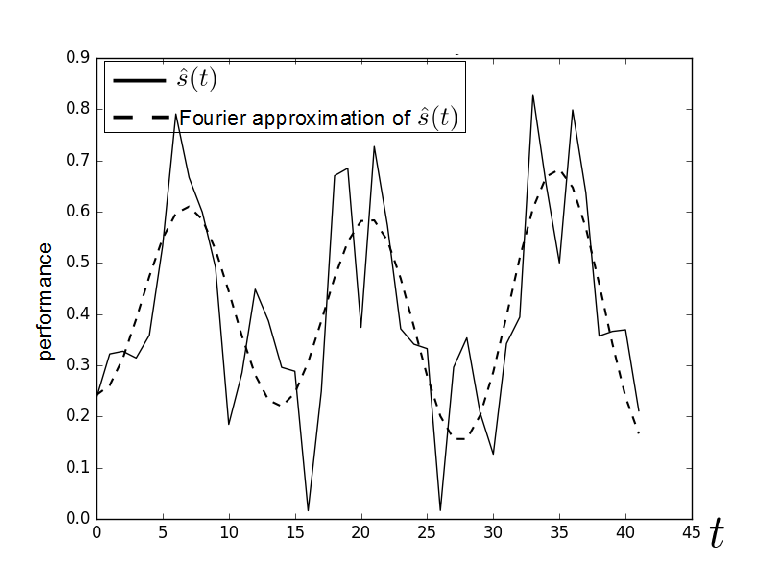
\includegraphics[width=10cm]{images/sample-fig.png}
	\caption{Contoh gambar.}
	\label{Fig: Contoh gambar}
\end{figure}

Contoh gambar terlihat pada Gambar \ref{Fig: Contoh gambar}. Gambar diambil dari \cite{wibowo2016clustering}.

\section{Penulisan Tabel}
\begin{table}[h]
	\caption{tabel ini}
	\vspace{0.5em}
	\centering
	\begin{tabular}{|c|c|c|}
		\hline
		ID & Tinggi Badan (cm) & Berat Badan (kg) \\
		\hline \hline
		A23 & 173 & 62 \\
		A25 & 185 & 78 \\
		A10 & 162 & 70 \\ \hline
	\end{tabular}
	\label{Tab: Tabel Tinggi Berat}
\end{table}
Contoh penulisan tabel bisa dilihat pada Tabel \ref{Tab: Tabel Tinggi Berat}.

\section{Penulisan formula}
Contoh penulisan formula
\begin{equation}
L_{\psi_z} = \{ t_i \mid v_z(t_i) \le \psi_z \}
\end{equation}

Contoh penulisan secara \textit{inline}: $\mathit{PV = nRT}$. Untuk kasus-kasus tertentu, kita membutuhkan perintah "mathit" dalam penulisan formula untuk menghindari adanya jeda saat penulisan formula.

Contoh formula \textbf{tanpa} menggunakan "mathit": $PVA = RTD$

Contoh formula \textbf{dengan} menggunakan "mathit": $\mathit{PVA = RTD}$



\section{Contoh list}
Berikut contoh penggunaan list
\begin{enumerate}
	\item First item
	\item Second item
	\item Third item
\end{enumerate}